\chapter{Two--Component Relativistic Electronic Structure Theory}
\label{ch:2CEST}


\section{The Exact Two--Component Hamiltonian}
\label{sec:X2C}

The problem of the diachoimy between the electronic and positronic states of the Dirac
equation may be attributed to the $c \op{\vc{p}} \cdot \vc a$ terms which couple the 
large and small components of the bispinor in \cref{eq:DiracHam}. In an attempt
to decouple these equations, we may perform a similarity transformation under an operator $\op{U}$, such that
\todo{cite}
\begin{equation}
\label{eq:FW}
\op h^D \mapsto \op h^\TwC  = \op U \op h^D \op U^{-1} = \begin{bmatrix} \op h^+ & 0 \\ 0 & \op h^- \end{bmatrix}.
\end{equation}
where both $\op h^+$ and $\op h^-$ are effective 2C operaters (i.e. they act on spinors).
In general, $\op U$ is referred to as a Foldy-Wouthuysen (FW) transformation \todo{cite}.
In essence, the FW transformation convolves the information contained in the large and small
component of the bispinor such that solution of \cref{eq:DiracEq} amounts to solving two decoupled 
differential equations,
\begin{align}
\op h^\pm \ket{ \phi^\pm (t) } = \ii \partial_t \ket{\phi^\pm (t)}, \qquad \op U \ket{\psi} = \begin{bmatrix} \ket{\phi^+} \\ \ket{\phi^-} \end{bmatrix}.
\end{align}
As such, the spectrum of $\op h^+$ and $\op h^-$ are given by
\begin{equation}
\mathrm{spec}(\op h^+) = (-c^2,\infty), \quad 
\mathrm{spec}(\op h^-) = (-\infty,-2c^2).
\end{equation}
In the case of a free electron, we obtain 
\begin{equation}
\label{eq:NWRep}
\op v = 0 \quad \Longrightarrow \quad \op h^\TwC = \vc b \sqrt{1 + \op p^2},
\end{equation}
which is known as the Newton--Wigner representation of the Dirac equation \todo{cite}. Even in the case
when $\op v \neq 0$, the FW transformation is possible, only one is not able to write down a closed
form expression such as \cref{eq:NWRep}, and power series approximations must be made in order to make
use of them in practical calculations 
\footnote{It is actually in the FW transformation in the presence of the scalar nuclear  potential 
that we are able to define terms like ``spin--orbit" coupling and the mass--velocity correction. The Dirac Equation need not know explicitly 
about these effects and accounts for them implicity through the coupling of the large and small components
of the electronic wave function. These terms which we typically associate with relativistic effects are in fact
terms in a series expansion which is only good in the non--relativistic limit.}
\todo{cite}. 
This series expansion may be avoided in the case of basis set calculations 
in the that problem of block--diagonalization of an operator in a basis representation is a well defined
numberical linear algebra problem.

To this end, we will account for relativistic effects using the exact two--component (X2C) method \todo{cite}.
The name X2C is a misnomer due to the fact that it is only ``exact" in the one electron case. There
exist many basis set methods to obtain effective 2C Hamiltoninans such as \cref{eq:FW} \todo{cite},
but the X2C method is an especially attractive method in that it is a one step transformation, rather than
an iterative procedure such as those involved in the Douglass--Kroll--Hess method and its variants \todo{cite}.
The X2C method operates under the assumption that there exists a linear, energy independent transformation which
links the large and small component of the electronic wave function. Expanding out the action of \cref{eq:DiracHam}
on a bispinor of the form \cref{eq:Bispinor}, we obtain the following relationship between the large and small components for positive energy 
solutions
\begin{equation}
  \label{eq:KineticBalance}
  \ket{\phi^S} = \frac{c \op{\vc p} \cdot \pauli{}}{(E - v + 2c^2)} \ket{\phi^L } \approx 
    \ket{\phi^{PL} } = \frac{\op{\vc p} \cdot \pauli{}}{2c} \ket{\phi^L },
\end{equation}
where $E$ and $v$ are the expectation values of the Dirac Hamiltonian and the potential operator in the bispinor, respectively.
The approximation on the right of \cref{eq:KineticBalance}, where we have defined the so--called pseudo large component, $\ket{\phi^{PL}}$,
holds in the non--relativstic limit ($E \approx v$, i.e. small momentum)
and is known as the kinetic balance condition for the small component of the electronic wave function \todo{cite}. 
Thus the action of the Dirac Hamitloninan on the bispinor may now be written as
\begin{equation}
\label{eq:ModDirac}
\begin{bmatrix}
\op v & \op T^\NR \\ \op T^\NR & \frac{1}{4c^2} \op W - \op T^\NR
\end{bmatrix}
\begin{bmatrix}
\ket {\phi^L} \\ \ket{\phi^{PL}}
\end{bmatrix}
\end{equation}
where $\op T^\NR$ is the non--relativistic kinetic energy operator of \cref{eq:SpinorKinMom}. $\op W$ is a transformed
potential operator given by
\begin{equation}
\op W = (\op{\vc p} \cdot \pauli{}) \op v (\op{\vc p} \cdot \pauli{}).
\end{equation}
\Cref{eq:ModDirac} is known as the modified Dirac equation.

In a finite basis $\{ \chi_\mu \}$ with $\vert \{\chi_\mu \} \vert = N_b$, we may develop a Roothaan--Hall--like equation from \cref{eq:ModDirac}
such that
\begin{equation}
\label{eq:MDRH}
\vc H^\mathrm{MD} \vc C^\mathrm{MD} = \vc S^\mathrm{MD} \vc C^\mathrm{MD} \vc \epsilon^\mathrm{MD},
\end{equation}
where
\begin{align}
&\vc H^\mathrm{MD} =
\begin{bmatrix}
\vc v & \vc T^\NR \\ \vc T^\NR & \frac{1}{4c^2} \vc W - \vc T^\NR
\end{bmatrix},\\
%
&\vc S^\mathrm{MD} =
\begin{bmatrix}
\vc S & \vc 0 \\ \vc 0 & \frac{1}{2c^2} \vc T^\NR
\end{bmatrix},\\
%
&\vc \epsilon^\mathrm{MD} =
\begin{bmatrix}
\vc \epsilon^+ & \vc 0 \\ \vc 0 & \vc \epsilon^-
\end{bmatrix},
\end{align}
and the basis representations of these operators are given as in \cref{eq:OBBasisExp}. The superscripts
$+$ and $-$ on the orbital eigenvalues denote electronic and positronic eigenvalues, respectively.
$\vc C^\mathrm{MD}$ takes the block form
\begin{equation}
\vc C^\mathrm{MD} = \begin{bmatrix} \vc C^{L+} & \vc C^{L-} \\ \vc C^{PL+} & \vc C^{PL-} \end{bmatrix},
\end{equation}
such that we may construct a basis $\mathcal C = \mathcal C^+ \cup \mathcal C^-$ which approximately spans $\hilb H^\FrC$
with $\mathcal C^+ \cap \mathcal C^- = \emptyset$ and $\vert \mathcal C^+ \vert = \vert \mathcal C^- \vert = 2N_b$ via
\begin{align}
&\mathcal C^+ = \left\lbrace \ket{\psi_p} \in \mathcal C \text{ s.t. } \psi_p(\vc{x}) = \begin{bmatrix} \phi_p^{L+}(\vc{x}) \\ \phi_p^{PL+}(\vc{x}) \end{bmatrix} \right\rbrace,\\
&\mathcal C^- = \left\lbrace \ket{\psi_p} \in \mathcal C \text{ s.t. } \psi_p(\vc{x}) = \begin{bmatrix} \phi_p^{L-}(\vc{x}) \\ \phi_p^{PL-}(\vc{x}) \end{bmatrix} \right\rbrace,\\
&\phi_p^{L\pm,\sigma}(\vc{r})  = \sum_\mu C^{L\pm,\sigma}_{\mu p} \chi_\mu(\vc r), \\
&\phi_p^{PL\pm,\sigma}(\vc{r}) = \sum_\mu C^{PL\pm,\sigma}_{\mu p} \chi_\mu(\vc r). 
\end{align}
To decouple \cref{eq:MDRH},
the X2C method employs the use of a unitary operator in the basis represetation \todo{cite},
\begin{equation}
\label{eq:X2CTrans}
\vc U^\XtC = \begin{bmatrix} \vc Y_1 & - \vc X^\dagger \vc Y_2 \\ \vc X \vc Y_1 & \vc Y_2 \end{bmatrix},
\quad \vc Y_1 \ (\vc I + \vc X^\dagger \vc X)^{-\frac{1}{2}},  
\quad \vc Y_2 \ (\vc I + \vc X \vc X^\dagger)^{-\frac{1}{2}}.  
\end{equation}
such that $\vc X$ is constructed from the eigenvectors of \cref{eq:MDRH} by
\begin{equation}
\vc X = \vc C^{PL+} \left(\vc C^{L+}\right)^{-1}.
\end{equation}
An account on how to efficiently assemble $\vc X$ is given in reference \todo{cite}.
Given $\vc{X}$, \cref{eq:X2CTrans} may 
be constructed and in the limit that $\op v$ only contains one body operators, \cref{eq:ModDirac} is block diagonalized 
exactly,
\begin{equation}
  \label{eq:X2CHam}
\vc U^\XtC \vc H^\mathrm{MD} \vc U^{\XtC\dagger} = \begin{bmatrix} \vc h^\XtC & \vc 0 \\ \vc 0 & \vc h^- \end{bmatrix}.
\end{equation}
Here we have labelled $\vc h^\XtC$ as the positive energy block diagonal of the transformed hamiltonian. $\vc h^\XtC$ 
will serve as the source of the relativistic effects in the mean field methods used throughout this work.










\section{Two--Component Relativistic Mean Field Wave Functions}
\label{sec:MF2C}


The power of of the X2C method outlined in \cref{sec:X2C} is that it allows one
to cast mean--field relativistic electronic structure theory into a form which closely 
resembles non--relativistic theory. 
In the case where $\op v$ is an effective many--body potential in the context of mean field theory, the X2C method
dictates that the transformation only be performed using the density independent terms of the Fock operator \todo{cite},
i.e. $\op H^\mathrm{core}$ of \cref{eq:FockComponents}. Otherwise, the transformation described by $\vc U^\XtC$ would
have to be performed as each step of the wave function optimization procedure outlined at the end  of \cref{sec:HF};
rendering the method impractical. It is for this reason that the X2C is only exact in that case of a single electron
in an external potential; the effective many body terms in the mean field Fock operator are neglected in the 
relativistic treatment. To remedy this somewhat egregious approximation, $\vc h^\XtC$ is transformed in such a
way as to effectively include these many--body effects by way of the B\"{o}ttger \co{ check spelling} scaling,
\begin{equation}
  \label{eq:BScaling}
\vc h^\XtC \mapsto \vc \Lambda^{B\dagger} \vc h^\XtC \vc \Lambda^{B},
\end{equation}
where $\vc \Lambda^B$ is the sparse matrix of B\"{o}ttger scaling factors \cite{Boettger00_7809}. 
This scaling method
has become the field standard for approximately accounting for many--body relativistic effects in effective
2C relativistic methods \todo{cite?}.

With our restriction from the DCB to DC Hamiltonian,
the two--body part of the electronic Hamiltonian in the effective 2C framework
is the same as it was in the non--relativistic case, i.e. the mean--field operators
$\op J$, $\op K$ and $\op V^{xc}$ and their basis representations $\spvc J$, $\spvc K$ and $\spvc V^{xc}$, are the same as in 
\cref{eq:NRFockCompSpace,eq:FockCompAOBasis}. This is due to the fact that for the electronic
eigenvectors of \cref{eq:MDRH}, the X2C transformation also block diagonalizes the 
bispinor MO coefficients,
\begin{equation}
\begin{bmatrix} \vc h^\XtC & \vc 0 \\ \vc 0 & \vc h^- \end{bmatrix}
\begin{bmatrix} \vc C^\XtC & \vc 0 \\ \vc 0 & \vc C^- \end{bmatrix} =
\begin{bmatrix} \vc S & \vc 0 \\ \vc 0 & \vc S^- \end{bmatrix}
\begin{bmatrix} \vc C^\XtC & \vc 0 \\ \vc 0 & \vc C^- \end{bmatrix} 
\begin{bmatrix} \vc \epsilon^\XtC & \vc 0 \\ \vc 0 & \vc \epsilon^- \end{bmatrix}.
\end{equation}
In effect, this block diagonalization manifests in the same manner as \cref{eq:USCFEq}. 
Denoting the bispinor orbitals which may be expanded in terms of 
$\vc C^\XtC$ as
\begin{equation}
  \mathcal C^\XtC = \left\lbrace
  \psi_p(\vc r, \sigma) = 
  \begin{bmatrix} \phi^\alpha_i (\vc r) \alpha(\sigma) \\ \phi^\beta_i(\vc r) \beta(\sigma) \\ 0 \\ 0 \end{bmatrix} =
  \sum_\mu \begin{bmatrix} C_{\mu p}^{\XtC,\alpha} \alpha(\sigma)\\ C_{\mu p}^{\XtC,\beta}\beta(\sigma) \\ 0 \\ 0 \end{bmatrix} \chi_\mu(\vc{r}) \right\rbrace, 
\end{equation}
we may express the relativsitc 1RDM  (\cref{eq:Rel1RDM}) which can be constructed from a 
subset $\mathcal K_I^N \subset \mathcal C^\XtC$ as
\begin{equation}
  \label{eq:Rel2C1RDM}
  \overline{\gamma}^1(\vc{x}; \vc x')
    \sum_{i \in \mathcal K^N_I} 
    \begin{bmatrix} 
      \phi_i(\vc{x}) \phi_i^{*}(\vc{x}') & 0 \\ 0 & 0 
    \end{bmatrix}. 
\end{equation}
As such, we will introduce a quasi--relativistic 1RDM which simply removes the zeroed out portions of \cref{eq:Rel2C1RDM},
\begin{equation}
  \label{eq:QRel2C1RDM}
  \overline{\gamma}^1(\vc{x}; \vc x') \mapsto {\gamma}^1(\vc{x}; \vc x') =
    \sum_{i \in \mathcal K^N_I} 
      \phi_i(\vc{x}) \phi_i^{*}(\vc{x}').
\end{equation}
Using this definition of $\gamma^1$, we may define the analogus mean field operators exactly as in 
\cref{eq:FockComponents,eq:VXCBasis}, thus yielding the same expressions for $\vc J$, $\vc K$, and $\vc V^{xc}$.


The key difference between the X2C method and non--relativistic mean field methods is in the definition of
the core Hamiltonian. In the four--componenet treatment of relativistic theory, the density independent term
is described by the Dirac Hamiltonian in \cref{eq:DiracHam}. However, in the X2C method, the basis representation
of the core Hamiltoninan is simply given by $\vc h^\XtC$ in \cref{eq:X2CHam}. Thus the basis representation of
the Fock matrix for HF and KS mean field wave functions (X2C-HF and X2C-KS), respectively) are given by
\begin{alignat}{2}
  \label{eq:X2CHFRH}
  &\spvc F^\mathrm{X2C-HF} = \spvc h^\XtC + \spvc J - \spvc K         && 
    \quad \text{s.t.}\quad \spvc F^\mathrm{X2C-HF} \spvc C^\mathrm{X2C-HF} = \spvc S\, \spvc C^\mathrm{X2C-HF} \spvc \epsilon^\mathrm{X2C-HF}, \\
  \label{eq:X2CKSRH}
  &\spvc F^\mathrm{X2C-KS} = \spvc h^\XtC + \spvc J + \spvc V^{xc} &&
    \quad \text{s.t.}\quad \spvc F^\mathrm{X2C-KS} \spvc C^\mathrm{X2C-KS} = \spvc S\, \spvc C^\mathrm{X2C-KS} \spvc \epsilon^\mathrm{X2C-KS},
\end{alignat}
such that we may decompose into the Pauli components of the Fock matrix
\begin{align}
  &\vc F^{0} = \vc h^{\XtC,0} + \vc J^0 + \vc X^0, \\
  &\vc F^{k} = \vc h^{\XtC,k} +  \vc X^k,\qquad k\in \{1,2,3\},
\end{align}
where $\spvc F \in \{\spvc F^\mathrm{X2CHF}, \spvc F^\mathrm{X2CKS} \}$ and $\spvc X$ is $-\spvc K$ for X2C-HF
wave functions and  $\spvc V^{xc}$ for X2C-KS wave functions. Thus, unlike the non--relativistic case of 
\cref{eq:NRFockPauli} where the spin components of the Fock matrix are completely determined by the 1PDM, the 
X2C Fock matrix explicitly admits spin into its Pauli components through the Pauli components of the X2C
core Hamiltonian. As such, X2C Fock matrix is of the form \cref{eq:GSCFFock}, and thus a GSCF procedure 
must be used in general.













\section{An Efficient and Scalable Implementation of Non-Collinear Density Functional Theory}
\label{sec:NCDFT}

\subsection{Motivation}
\label{sec:NCDFT_Motiv}

DFT (\cref{sec:DFT}) has become the primary investigative tool for quantum chemical calculations
regarding systems at large, experimentally relevant scales. The primary reason
for its success has been its excellent balance of accuracy and computational
cost and the vast availability through the development of efficient and
reliable DFT software capable of leveraging the latest advances in
high--performance computing \cite{Genovese17_e1290}.  
Efficient and robust numerical integration techniques for the xc potential (\cref{eq:VXCBasis}) have been
thoroughly studied throughout the
years \cite{Becke88_2547,Jackson90_7453,Laming93_997,Johnson95_169,Frisch96_213,Reveles04_681,Sierka11_3097},
and their proper application is crucial to the practicality and applicability
of DFT methods.  The wide adoption of DFT in the scientific community as
a whole has enabled routine, \emph{ab initio} characterization of both ground
and excited state properties for large macromolecular systems such as those of
biological \cite{Payne14_3614,Mennucci17_294,Rega18_1126} and
materials \cite{Ceder06_659,Skylaris16_220901,Li16_165402,Li16_7255,Li16_1601307,Li17_161}
interest and their transient
behavior \cite{Li16_104107,Li16_935,Li16_4501,Li17_3958}.

% Spin and why its important in materials, etc
Recently, there has been a resurgence of interest in the materials community
for the development and design of materials which exploit properties of
electronic spin in their applications, such as magnetic materials, spintronic
devices, and catalytic active sites
\cite{Berdinsky02_603,Ullrich06_2285,Sanvito11_3336,Mouritsen16_299} .  As
such, there is a strong need for electronic structure theories that are capable
of treating electronic spins in large scale systems. Thus, motivated by its
success in other aspects of materials research, there has been a large emphasis
in recent years on the extension of existing DFT methods to properly
include electronic spin and spin interactions.

% Relativistic Theory!
At its core, a rigorous treatment of electronic spin and its interaction with
materials in quantum systems must be rooted in relativistic quantum mechanics
\cite{Dreizler84_353,Faegri07_book,Pyykko12_45,Wolf15_book}. 
As was discussed in \cref{sec:RELH}, the introduction
spin--couplings into the relativistic Hamiltonian has been demonstrated to yield profound
effects even in light elements \cite{Pyykko12_45}, which may be physically
realized in systems such as doped nanodiamonds which have recently been
recognized as  fantastic candidates for the next generation of spintronic
devices and $q$-bits in quantum
computers \cite{Proskuryakov12_226402,Gali17_081115,Awschalom10_8513,Obrien10_7285,Petta13_1174,Li16_165402}.
Due to this centralized importance in the treatment of electronic spin, there
has been a lot of effort in recent years to extend existing electronic
structure methods to include relativistic effects, chief among them being
extensions of DFT based methods in both the
ground \cite{Helgaker02_814,Liu03_597,Cheng07_104106,Saue11_1439} and
excited \cite{Jensen03_522,Liu04_6658,Saue09_2091,Li16_5379,Li17_2591}
electronic states.  
Relativistic analogues to the Hohenberg--Kohn
theorems require the exact energy functional not only to be a functional of the
electronic density, but also of the current
density \cite{Vignale95_485,Engel98_138,Faegri07_book,Ullrich04_20,Rajagopal96_book,Wolf15_book,Rasolt87_2360,Boeij07_174111,Gross07_100401,Gross08_245106}.
While some work has gone into the development of these types of
functionals \cite{Tozer08_074101,Colwell95_10095,Sandratskii98_91,Ullrich09_859,Gross13_156401,Furche12_164105,Teale15_4169},
the bulk of widely used exchange correlation functionals do not include these
effects due to the fact that their contribution is typically small. 


% Spin non--collinearity + retrofitting functionals in 2 / 4 C
One of the central challenges in relativistic DFT is in that the introduction
of spin couplings into the Hamiltonian necessarily introduce spin
non--collinearity  in the electronic density for open--shell systems, i.e the
spin magnetization vector is no longer restricted to coincide with the
$z$--axis (see \cref{sec:SpinSymm,sec:MF2C}). In this regard, unlike the collinear
theory, non-collinear DFT requires the functional to depend on scalar and magnetization
densities (\cref{eq:Densities}).
Unfortunately, density functionals commonly
employed in quantum chemistry have been developed for collinear densities, and
therefore, there is no straightforward way to employ them in non-collinear
systems.  
%
%In this context, any  non-collinear DFT generalization  needs also to
%pay particular attention on preserving the property that the self-consistent xc
%magnetic field cannot exert a net torque on the system as a whole (zero-torque
%theorem) \cite{Gyorffy01_206403}.  On the other hand,  the local torque does not
%need to vanish identically at every point in space, since this local
%contribution is required to obtain accurate spin dynamics and a proper
%time-evolution of the
%magnetization\cite{Gyorffy01_206403,Gyorffy03_354,Gross07_196405,Frisch07_125119,Frisch12_2193,Scuseria13_035117,Li17_2591}.
%
In this context, any generalization of collinear DFT to non-collinear densities
must adhere to the so called zero--torque theorem \cite{Gyorffy01_206403},
namely that the xc magnetic field (see \cref{apx:ZeroTorque} \cref{eq:xcMagField}) cannot
exert a net torque on the magnetization density. However, if such a generalization
does not admit local torque by the xc magnetic field, one cannot resolve proper
time--evolution of the magnetization density in the absense of fields
\cite{Gyorffy01_206403,Gyorffy03_354,Gross07_196405,Frisch07_125119,Frisch12_2193,Scuseria13_035117,Li17_2591}.
%
Several efforts have been made to adapt common density functionals
developed for collinear densities for use 
relativistic calculations in this manner, both in the context of relativistic
two-component \cite{Wullen02_779,Liu03_597,Ziegler04_12191,Liu05_144101,Frisch07_125119,Frisch12_2193,Scuseria13_035117,Li17_2591}
and four-component
\cite{Helgaker02_814,Saue03_10418,Servedio99_23,Liu03_597,Engel04_012505}
methods.  
However, in stark contrast to its non--relativistic collinear counterpart, no work has gone into developing highly optimized
numerical integration techniques for these relativistic DFT methods. Thus, in this work, we outline an efficient algorithm 
and practical considerations for the integration of the xc potential in non--collinear relativistic DFT.















\subsection{Assembly of the Exchange--Correlation Potential for Spinor Densities}

In this section, we examine the integration and assembly of the $\tilde E^{xc}$ (\cref{eq:KSXC_func})
dependent terms of the KS Fock matrix using a spinor density (see
\cref{sec:MF2C}).  In this work, we will limit our discussion to those
functionals which may be characterized under the hybrid generalized gradient
approximation (hybrid GGA), where $\tilde E^{xc}$ takes the form
\begin{equation}
  \label{eq:XCFUN}
\tilde E^{xc}[\gamma^1] = E^{GGA}[\vc\rho^1,\nabla\vc\rho^1] - c_{x}K[\gamma^1] .
\end{equation}
Here, the full $\tilde E^{xc}$ has been partitioned into a pure GGA exchange correlation functional, $E^{GGA}$, 
which is a functional of the electronic density ($\vc \rho^1$) and its gradient (see \cref{eq:Densities}),
and a scaled ($c_x \in [0,1]$) Hartree--Fock exchange energy (\cref{eq:ExchFunc}).
In general, the exchange correlation contribution to the
electronic energy may be written as an integral over an exchange correlation (xc) integration kernel, $f$,
\begin{equation}
  \label{eq:EXCEVAL}
E^{GGA}[\vc \rho^1, \nabla \vc \rho^1] = \int \mathrm{d}^3 \vc r \text{  }f(\{ U(\vc{r}) \}) ,
\end{equation}
where we have introduced a set of auxiliary ``U"--variables, $\{U(\vc{r})\}$, upon which
the xc kernel depends. These need not be the density variables ($\vc \rho^1, \nabla \vc \rho^1$) directly,
which we will refer to as ``V"--variables, $\{V(\vc{r})\}$, but rather have complete flexibility in
functional form. In non--relativistic, spin--polarized (collinear) DFT, these sets of variables
may be defined as
\begin{equation}
  \label{eq:Vcol}
  \{ V^{col}(\vc{r}) \} = \{ \rho^{1,\saa}(\vc{r}), \rho^{1,\sbb}(\vc{r}), \nabla \rho^{1,\saa}(\vc{r}), \nabla \rho^{1,\sbb}(\vc{r}) \} 
\end{equation}
and
\begin{equation}
  \label{eq:Ucol}
  \{ U^{col}(\vc{r}) \} = \{ \rho^{1,\saa}(\vc{r}), \rho^{1,\sbb}(\vc{r}), \varphi^\saa(\vc{r}), \varphi^\sab(\vc{r}), \varphi^\sbb(\vc{r}) \}
\end{equation}
where
\begin{equation}
  \varphi^{\sigma\sigma'}(\vc{r}) = \nabla \rho^{1,\sigma\sigma}(\vc{r}) \cdot \nabla \rho^{1,\sigma'\sigma'}(\vc{r})
\end{equation}
The practical utility for the use of these two separate sets of variables 
is especially apparent in the context of two--component density functional theory
as it allows for a simple retrofitting of standard xc functionals for relativistic calculations
by simply redefining the transformations from the V variables of relativistic theory. 

Define the scalar and magnetization densities as in \cref{eq:Densities}, we may define 2C analogues
to the collinear auxillary variables as
\begin{align}
  \label{eq:NCAuxVar}
  &\{ V^{NC}(\vc{r}) \} = \{ \rho^{1,0}(\vc{r}), \mathbf{m}(\vc{r}), \nabla \rho^{1,0}(\vc r), \nabla \mathbf{m}(\vc{r}) \} \\
  &\{ U^{NC}(\vc{r}) \} = \{ n^+(\vc{r}), n^-(\vc{r}), \varphi^{++}(\vc{r}), \varphi^{+-}(\vc{r}), \varphi^{--}(\vc{r}) \}
\end{align}
where we have used $NC$ to denote non--collinearity. The connection between $\{U^{col}\}$ and $\{U^{NC}\}$
is clear by making the substitution $\alpha \leftrightarrow +$ and $\beta \leftrightarrow -$. 
$\{V^{col}\}$ and $\{V^{NC}\}$ may be related by recognizing $\{\rho^{1,\saa},\rho^{1,\sbb}\}$ as the diagonal contributions
of the spinor density, and thus
\begin{equation}
  \{\rho^{1,\saa}(\vc{r}), \rho^{1,\sbb}(\vc{r})\} \mapsto \{\rho^{1,0}(\vc{r}), \mathbf{m}^{col}(\vc{r})\}
\end{equation}
where $\mathbf{m}^{col}(\vc{r}) = \{0,0,\rho^{1,3}(\vc{r})\}$. Given the components of the spinor density matrix,
spatial evaluation of the V--variables is given by (\cref{eq:DenMatEval})
\begin{alignat}{2}
  \label{eq:VVarEval}
  \rho^{1,K}(\vc{r}) &= \sum_{\mu\nu} \mathrm{Re}[P^K_{\mu\nu}] \chi_\mu(\vc{r}) \chi_\nu(\vc{r}) \quad && K \in{0,1,2,3}\\
  \nabla\rho^{1,K}(\vc{r}) &= 2\sum_{\mu\nu} \mathrm{Re}[P^K_{\mu\nu}] \chi_\mu(\vc{r}) \nabla\chi_\nu(\vc{r})\quad && K \in{0,1,2,3}
\end{alignat}
where the matrices $\vc P^K$ are defined as in \cref{eq:1PDM} and $\mathrm{Re}[x]$ denotes the real part of $x$. Remark that the evaluation of $\{V^\NC(\vc{r})\}$ may then be practically 
evaluated using strictly real arithmetic.

Given a transformation, $\{ V^{NC}(\vc{r}) \} \mapsto \{U^{NC}(\vc{r})\}$, it is possible to perform practical
density functional calculations using standard implementations of collinear xc functionals, such
as those provided by \texttt{libxc} \cite{Burnus12_2272,Marques18_1}. However, defining such a transformation is not 
a trivial task, as the added spin degrees of freedom in the non--collinear spinor density and
Fock matrix must obey to stricter conditions than their collinear counterparts, such as orientation
invariance and adhering to the zero--torque theorem for the xc potential \cite{Gyorffy01_206403}.
Several definitions of the generalized density variables have been proposed \cite{Wullen02_779,Ullrich05_073102,Frisch07_125119,Frisch12_2193,Scuseria13_035117}.
In this work, we utilize the transformation method which meets such conditions from Ref.\cite{Li17_2591} 
\begin{subequations}
  \label{eq:NCtrans}
  \begin{align}    
    n^\pm(\vc{r})        & = \rho^{1,0}(\vc{r}) \pm \vert\mathbf{m}(\vc{r})\vert\\
     \varphi^{\pm\pm}(\vc{r}) & = D^{00}(\vc r)   + \sum_{k=1}^3 D^{kk} (\vc r) 
                           \pm f_{\nabla}(\vc{r})\sqrt{ \sum_{k=1}^3 D^{0k}(\vc{r})^2} \\
     \varphi^{+-}(\vc{r})      & = D^{00} (\vc r)
                           - \sum_{k=1}^3 D^{kk} (\vc r)
  \end{align}
\end{subequations}
where
\begin{align}  
  f_{\nabla}(\vc{r}) & = sgn\left(\nabla\rho^{1,0} (\vc{r}) \cdot \left(\sum_{k=1}^3 \nabla \rho^{1,k}(\vc r) \rho^{1,k}(\vc r) \right)\right) \\
  D^{KL} (\vc{r})      &  = \nabla\rho^{1,K} (\vc{r}) \cdot  \nabla \rho^{1,L} (\vc{r})  
\end{align} 
Using this set of transformations, we may define an electronic energy and Fock matrix which has no dependence
on the global orientation of $\mathbf{m}(\vc{r})$ and which satisfies the zero torque theorem (see \cref{apx:ZeroTorque}) for
the xc potential within in the GGA framework.

In the limit of small $\mathbf{m}(\vc{r})$ ($\lvert \mathbf{m}(\vc{r}) \rvert <
10^{-12}$, in this work), the transformations outlined in \cref{eq:NCtrans}
yield numerically unstable expressions for the exchange correlation
potential \cite{Li17_2591}. Thus one must define another set of transformations
for practical implementations of non--collinear DFT to ensure proper
convergence in the limit of small $\mathbf{m}(\vc{r})$. In summary, this change
for small $\mathbf{m}(\vc{r})$ may be described by the following substitutions
in \cref{eq:NCtrans},
\begin{subequations}
  \label{eq:smallTrans}
%  \begin{align}  
%    n^\pm(\vc{r})        & = \frac{1}{2}\rho^S(\vc{r}) \pm \frac{1}{2} \left( \frac{1}{3}\sum_k \rho^k(\vc{r}) \right) \\ 
%    \varphi^{\pm\pm}(\vc{r}) & = \frac{1}{4}\nabla\rho^S (\vc{r})\cdot \nabla\rho^S (\vc{r})  \\
%                         & + \frac{1}{4}\sum_k \nabla\rho^k (\vc{r}) \cdot \nabla\rho^k (\vc{r}) \nonumber \\
%                         & \pm \frac{f_{\nabla}(\vc{r})}{2} \left( \frac{1}{3}\sum_k D^{Sk}  (\vc{r}) \right) \nonumber \\
%    \varphi^\pm(\vc{r})      & = \frac{1}{4}\nabla\rho^S (\vc{r})\cdot \nabla\rho^S (\vc{r}) \\ 
%                         & - \frac{1}{4}\sum_k \nabla\rho^k (\vc{r}) \cdot \nabla\rho^k (\vc{r}) \nonumber
%  \end{align}
\begin{align}
  \vert \mathbf{m}(\vc{r}) \vert   &\mapsto m_s(\vc r) = \frac{1}{3}\sum_{k=1}^3 \rho^{1,k}(\vc{r}),\\
  \sqrt{ \sum_{k=1}^3 \left( D^{0k} (\vc{r}) \right)^2} &\mapsto \nabla \rho^{1,0}(\vc r) \cdot \nabla m_s(\vc r).
\end{align}
\end{subequations}
Using these mappings ensures no orientation dependence of $\mathbf{m}$ while maintaining numerical stability
in the resulting expression for the xc potential. While \cref{eq:smallTrans} formally violates the zero
torque theorem, its influence on the over all nature of the electronic density has been shown to be 
negligible \cite{Li17_2591}.

Differentiating \cref{eq:EXCEVAL} with respect to the elements of the density matrix, we obtain for \cref{eq:VXCBasis} 
(or more specifically its Pauli components)
\begin{equation}
  V^{xc,L}_{\mu\nu} = V^{GGA,L}_{\mu\nu} - c_{HF} K^L_{\mu\nu},\quad L \in \{0,1,2,3\},
\end{equation}
where $\spvc K$ is the HF exchange matrix (\cref{eq:HFX_mat}) and
\begin{align}
  \label{eq:VXCGGA_eval}
V^{GGA,K}_{\mu\nu} &= \sum_{\Gamma \Gamma'} \int \mathrm{d}^3 \vc r \text{  }
  \frac{\partial f }{\partial U^{\NC,\Gamma}(\mathbf{r})}
  \frac{\partial U^{\NC,\Gamma}(\mathbf{r})}{\partial V^{\NC,\Gamma'}(\mathbf{r})}
  \frac{\partial V^{\NC,\Gamma'}(\mathbf{r})}{\partial P^{K}_{\mu\nu}} \\ &= \nonumber \int \mathrm{d}^3 \vc r \text{  } V^{GGA,K}_{\mu\nu}(\vc{r})
\end{align}  
where the partial derivatives of $f$ are the same as in collinear DFT, and the partial derivatives of $\{V^\NC(\vc{r})\}$ may be
identified through differentiating \cref{eq:VVarEval} for a particular spin component. We refer the reader to the Appendix
of Ref.\cite{Li17_2591} for explicit expressions for the Jacobians between $\{U^\NC(\vc{r})\}$ and $\{V^\NC(\vc{r})\}$ .

In practice, \cref{eq:EXCEVAL,eq:VXCGGA_eval} are evaluated numerically using a molecular quadrature scheme
\cite{Becke88_2547,Jackson90_7453,Laming93_997,Johnson95_169,Frisch96_213,Reveles04_681,Sierka11_3097},
\begin{align}
  &E^{GGA}[\vc \rho,\nabla\vc \rho] \approx \sum_i w(\vc{r}_i) f(\{U(\vc{r}_i)\}) \label{eq:EXCGGA_num}\\
  &V^{GGA,K}_{\mu\nu} \approx \sum_i w(\vc{r}_i) V^{GGA,K}_{\mu\nu}(\vc{r}_i) \label{eq:VXCGGA_num}
\end{align}
where $\{w(\vc{r}_i)\}$ is a set of quadrature weights. 
In this work, we utilize the Becke multi-center numerical integration scheme
\cite{Becke88_2547}, where the integral is evaluated on series of overlapping
atomic centered grids, transformed, through their weights, into ``fuzzy'',
overlapping, and analytically continuous cells instead.  We refer the
reader to a more thorough discussion regarding specific
details of the numerical integration \cite{Becke88_2547,Frisch96_213}.
%%%%% We can put this back if we need to
%Here, we simply remark that the hallmark of the Becke integration scheme is that the the molecular integrand is decomposed
%into a sum over overlapping atomic integrands,
%\begin{equation}
%  \mathcal{I} = \sum_A \mathcal{I}_A \qquad \mathcal{I} \in \{ E_{xc}^{GGA}, V^{GGA,I}_{\mu\nu} \}
%\end{equation}
%where the atomic integrands, $\mathcal{I}_A$ can be performed using standard spherical integration techniques.
%%%%%%
The evaluation of \cref{eq:EXCGGA_num} is straight forward as it is a scalar function. In the spirit of the intermediates used
in Ref.\cite{Sierka11_3097}, by substituting the definitions of the partial derivatives of the U and V variables, we arrive
at a concise expressions for assembly of \cref{eq:VXCGGA_num} 
\begin{align}
&V^{GGA,K}_{\mu\nu} = \sum_i Z^K_\mu(\vc{r}_i) \chi_\nu(\vc{r}_i) + Z^K_\nu(\vc{r}_i) \chi_\mu(\vc{r}_i) \label{eq:VXC_point_update}\\
  &Z^K_\mu(\vc{r}) = w(\vc{r})
    \left(
      \frac{1}{2} \mathcal{Z}^K_{\rho}(\vc{r}) \chi_\mu(\vc{r}) + \sum_\xi \mathcal{Z}^K_{\nabla,\xi}(\vc{r}) \nabla_\xi \chi_\mu(\vc{r})
    \right) \label{eq:ZKmu}
\end{align}
where $\xi \in \{x,y,z\}$ and
\begin{subequations}
\begin{align}
&\mathcal{Z}^K_{\rho}=     \frac{\partial f}{\partial \rho^{1,K}} =
                                     \begin{cases}
  \left( \dfrac{\partial f}{\partial n^+} + \dfrac{\partial f}{\partial n^-} \right) & K = 0 \\[12pt]
  \left( \dfrac{\partial f}{\partial n^+} - \dfrac{\partial f}{\partial n^-} \right) \mathscr K^{K} & K \neq 0 \\
                                     \end{cases}
\end{align}
\label{eq:ZrhoVar}
\end{subequations}

\begin{subequations}
\label{eq:ZvarphiVar}
\begin{align}
&\mathcal{Z}^K_{\nabla,\xi} = \frac{\partial f}{\partial \nabla_\xi \rho^{1,K}} = \begin{cases}
                                                          \nabla_\xi\rho^{1,0}    \left(  \dfrac{\partial f}{\partial \varphi^{++}} + \dfrac{\partial f}{\partial \varphi^{+-}} + \dfrac{\partial f}{\partial \varphi^{--}} \right)  
                                                          + \sum_{k=1}^3 \nabla_\xi \rho^{1,k} \mathscr H^k 
                                                          \left( \dfrac{\partial f}{\partial \varphi^{++}} - \dfrac{\partial f}{\partial \varphi^{--}} 
                                                          \right)                                                          
                                                          & K= 0 \\[8pt]                                                                                                        
                                                          \nabla_\xi\rho^{1,0} \mathscr H^K  \left( \dfrac{\partial f}{\partial \varphi^{++}} - \dfrac{\partial f}{\partial \varphi^{--}} \right) 
                                                          + \nabla_\xi\rho^{1,K}
                                                          \left(\dfrac{\partial f}{\partial \varphi^{++}} - \dfrac{\partial f}{\partial \varphi^{+-}} + \dfrac{\partial f}{\partial \varphi^{--}}
                                                           \right)
                                                          & K \neq 0
                                                        \end{cases}                                                                                                                                     
\end{align}
\end{subequations}
where we have dropped the explicit dependence on $\vc r$ for brevity. To consolidate the transformation rules of 
\cref{eq:NCtrans,eq:smallTrans}, we now define
\begin{subequations}
\begin{align}
&\mathscr K^K = 
\begin{cases}
  \dfrac{\rho^{1,K}}{\vert \mathbf{m} \vert} & \text{(Significant }\mathbf{m}\text{)} \\[20pt]
  \dfrac{1}{6} & \text{ (Small }\mathbf{m}\text{)} \\[12pt]
\end{cases}\\
&\mathscr H^K = 
\begin{cases}
  \dfrac{f_\nabla D^{0K} }{\sqrt{\sum_{k=1}^3 \left(D^{0k}\right)^2   }} & \text{(Significant }\mathbf{m}\text{)} \\[20pt]
  \dfrac{f_\nabla}{6} & \text{(Small }\mathbf{m}\text{)} \\[12pt]
\end{cases}
\end{align}
\end{subequations}


\subsection{Implementation}
\label{sec:NCDFT_IMPL}

On modern computing architectures, there are three primary facets one must consider when developing high--performance
scientific software: parallelism, cache utilization, and exploitation of micro-architecture specific floating point
operations ($\mu$-ops) such as single instruction--multiple data (SIMD) and fused multiply--add (FMA) operations. 
We refer the reader to the work of Goto, \emph{et al} \cite{Goto08_TOMS12} for an excellent discussion of these considerations in the context of matrix operations.
In the context of density functional theory, maximal exploitation of computational cache
and $\mu$-ops is achieved through batching groups of integration points together to maximize screening capability and
memory contingency. 
There exist many batching schemes for various molecular integration quadratures in the 
literature \cite{Becke88_2547,Jackson90_7453,Laming93_997,Johnson95_169,Frisch96_213,Reveles04_681,Sierka11_3097}.
We provide the following discussion without loss of generality.

As the point--wise
function evaluations required for numerical integration are completely independent, it constitutes what is called an
\emph{embarrassingly parallel task}, i.e. no communication is required between the independent operations and thus
one should expect near linear speedup with the number of processors used. 
In the context of electronic structure theory,
the final two facets can usually be addressed through the use of highly optimized linear algebra software, such as
the optimized BLAS (basic linear algebra subroutines) implementations offered OpenBLAS \cite{Qing13_ICHPC25,Yunquan12_PDS684} BLIS \cite{vanDeGeijn15_TOMS14} and Intel--MKL \cite{MKL}. 
However, blind application of such software without careful consideration will often yield sub-optimal results,
thus it is often the case that one must perform some level of algorithmic rearrangement to maximally utilize
such capability. 
To demonstrate this point, we examine the assembly of the exchange correlation potential
in \cref{eq:VXC_point_update}.
One may immediately recognize that the operation on the left of \cref{eq:VXC_point_update}
is a sum over symmetric rank--2 updates (SYR2) of column vectors, $\mathbf{z}$ and $\boldsymbol{\chi}$,
i.e.
\begin{equation}
\label{eq:VXC_SYR2}
\mathbf{V}^{GGA,I} = \sum_i \mathbf{z}^I_i \boldsymbol{\chi}_i^T + \boldsymbol{\chi}_i \left(\mathbf{z}^I_i\right)^T ,
\end{equation}
where $\mathbf{z}_i^I$ and $\boldsymbol{\chi}_i$ are of length of the number of basis functions, $N_b$. While \cref{eq:VXC_SYR2}
is a valid scheme for the assembly of \cref{eq:VXC_point_update}, for large $N_b$ this scheme will be drastically sub-optimal.
This is due to the fact that, for large $N_b$, $\mathbf{V}^{GGA,I}$, $\mathbf{z}_i^I$ and $\boldsymbol{\chi}_i$ occupy a significant
portion of the computational caches for each point. This means that the probability of the program attempting to access
a memory address, i.e. an element of $\mathbf{z}_i^I$ or $\boldsymbol{\chi}_i$, between integration points and finding that it does not
currently reside in the cache, i.e. a ``cache miss", is rather high relative to other memory access patterns. This yields a
large degradation in performance as whenever a cache miss occurs, the program must then move that address in some manner to
the cache from main memory before it can perform any operations on it. Moving data to and from main memory is disproportional
more expensive than floating point operations, thus it must be kept to a minimum to obtain
optimal efficiency.


\begin{figure}[t!]
\begin{center}
\resizebox{3.0in}{!}{%
  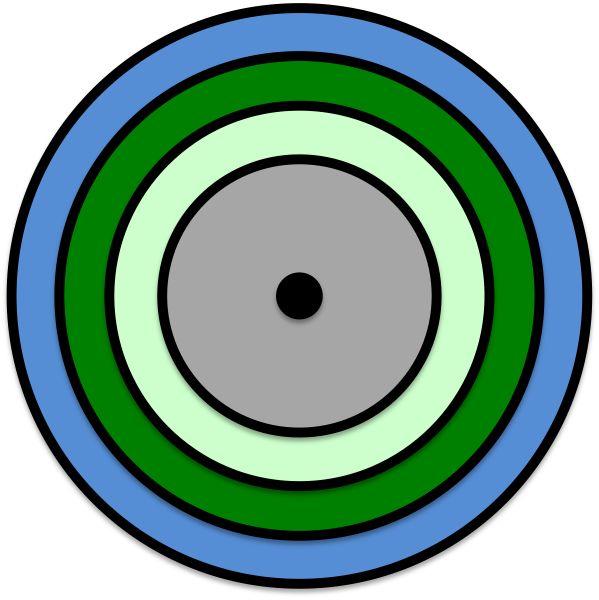
\includegraphics{Batches.png}
}
\end{center}
\caption{Pictorial representation of the integrand macrobatching scheme for the xc potential integration. 
Each of the colored regions represent a set of Lebedev spheres over several radial quadrature points, with the 
solid black dot representing the atomic nucleus. In the batching scheme, the scalar and matrix integrands
are evaluated over the entire batch simultaneously to improving caching and $\mu$-op behaviour.
}
\label{fig:Batching}       % Give a unique label
\end{figure}

\begin{figure}
\begin{center}
\resizebox{3.25in}{!}{%
  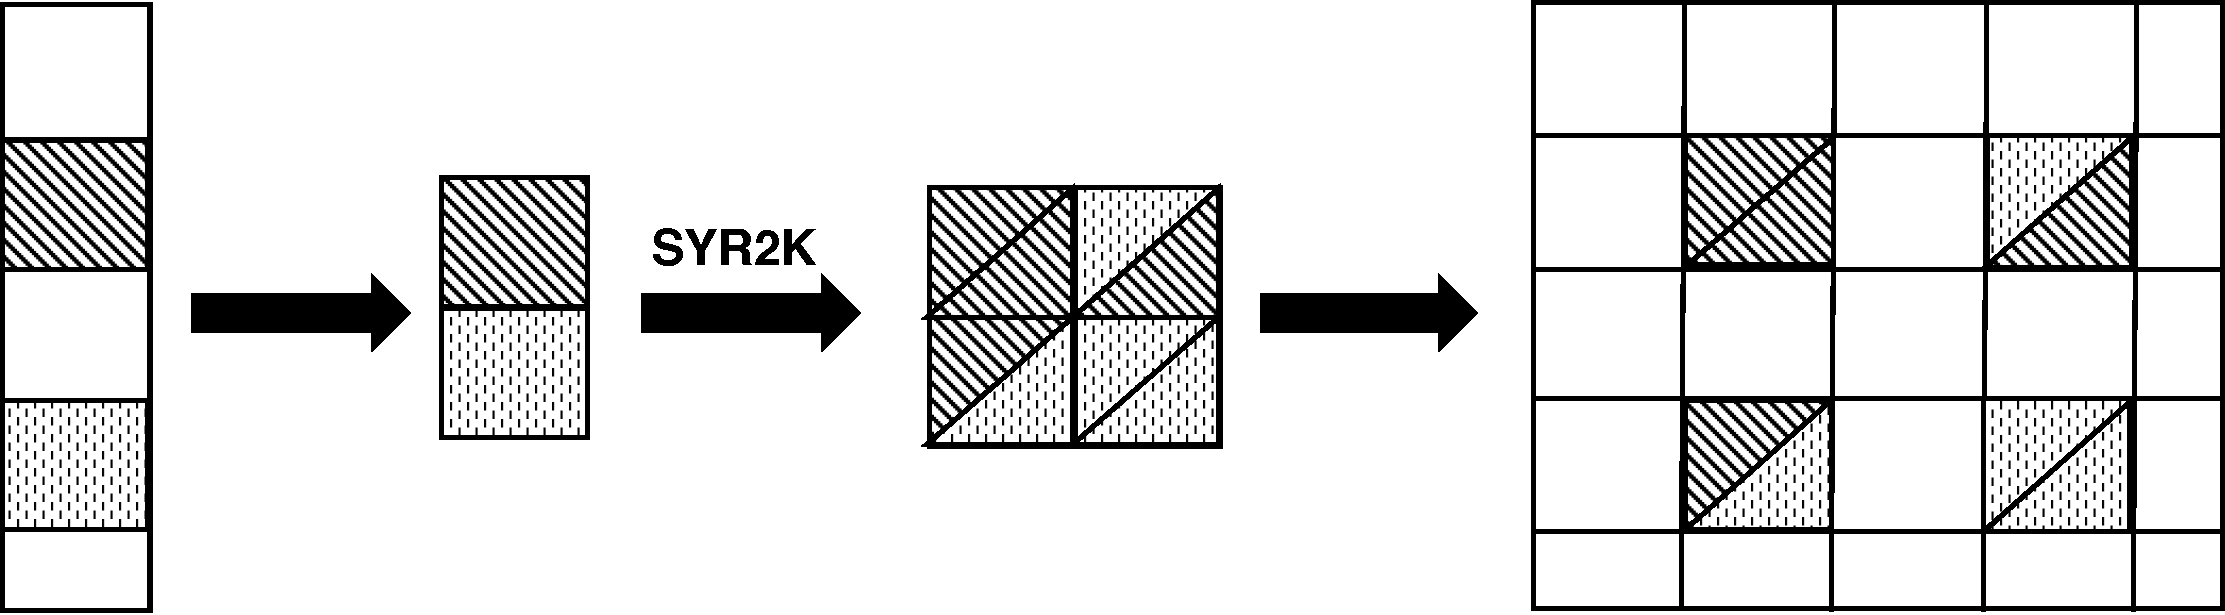
\includegraphics{Scheme2.pdf}
}
\end{center}
\caption{Pictorial representation of the screening and updating scheme for each
batch in the numerical integration of the xc potential.  A list of significant
basis functions in the batch (colored patterns in the figure) is selected and
than partitioned out for integration of that batch.  The accumulation of the
matrix integrand over the batch is evaluated by SYR2K  and then the final,
unscreened result is updated as shown. This scheme allows for only sequentional
memory access in the performance critical section of the integration and is
responsible for drastic performance increases.}
\label{fig:Integration}       % Give a unique label
\end{figure}

We may instead factor out a portion of the sum in \cref{eq:VXC_SYR2} such that
we may partition it into sum over batches of points.  In this work, we utilize a
macrobatch approach \cite{Frisch96_213}, where the grid points of each atoms are
grouped  into Lebedev spheres \cite{Lebedev77_99} of several radial quadrature points. This scheme
is pictorially represented in \cref{fig:Batching}. Denoting the set of all batches
as $\mathscr B$, we obtain

\begin{align}
\label{eq:VXC_SYR2K}
\mathbf{V}^{GGA,I} &= \sum_{S_j \in \mathscr B} \left(\sum_{i\in S_j} \mathbf{z}^I_i \boldsymbol{\chi}_i^T + \boldsymbol{\chi}_i \left(\mathbf{z}^I_i\right)^T \right) \nonumber \\
&= \sum_{S_j \in \mathscr B} \mathbf{Z}^{I(j)} \left(\mathbf{X}^{(j)}\right)^T + \mathbf{X}^{(j)} \left(\mathbf{Z}^{I(j)}\right)^T
\end{align}
where
\begin{equation}
\mathbf{Y}^{(j)} = \begin{bmatrix} \mathbf{y}_1 & \mathbf{y}_{2} & \cdots & \mathbf{y}_i & \cdots &\mathbf{y}_{\vert S_j \vert} \end{bmatrix} \quad \forall i\in S_j,
\end{equation}
and $\mathbf{y}$ is either $\mathbf{z}$ or $\boldsymbol{\chi}$. \Cref{eq:VXC_SYR2K} is a sum over symmetric rank--2$k$ updates (SYR2K), where $k = \vert S_j \vert$. By tuning
$k$, one improves caching behavior dramatically. This is due to the fact that optimized implementations of SYR2K operations utilized efficient block
operations to optimize the flow of data to and from the computational caches. 
%  \todo{make a table / plot of cache misses + wall time for SYR2 and SYR2K}.}
 Similar schemes may
developed for the evaluation of the V variables (\cref{eq:VVarEval}) over batches using optimized matrix--matrix multiplication routines. However, while the caching behavior
is improved with increasing $k$, this is not the only consideration one needs take into account when partitioning the integration grid into batches.

The scheme in \cref{eq:VXC_SYR2K} may be further improved by recognizing the fact  that the basis functions typically used for molecular calculations carry 
a degree of spatial locality. 
A pictorial representation of the screening and updating scheme is given in \cref{fig:Integration}.
For each batch, we create a list of basis functions
that effectively overlaps it (colored subset of basis functions in \cref{fig:Integration}). 
This list of significant basis functions will be different for
each batch, but the number of basis
functions in each list becomes independent of size
for sufficiently large molecules, given the  spatial localization nature of Gaussian atomic centered basis sets.
%As such, not every basis function need be evaluated for every batch depending on the distance of the basis function to the points in the
%batch. Deciding which basis functions need to be evaluated are dependent on the characteristics of the basis set. \todo{explain / cite how we screen}. 
This reduced list of basis, evaluated for all points in the batch, is stored in contiguous blocks of memory, and used (along with the corresponding submatrices of the density-matrix, when required) for the evaluation of the potential, $\mathbf{Z}$ (see \cref{eq:ZImu}), by exploiting a sub-sequential series of vectorized operations.
An important note here is that the maximum values for the batch of basis functions, $\chi_{max}(batch)$, and potential, $Z_{max}(batch)$, can be used to screen the entire contribution of the points in the batch to the integration. In this case, the integration can move to the next batch, avoiding the rank-2k update, that is the computationally most expensive part of the process,  without loosing accuracy.
Otherwise, recognizing that $\mathbf{Z}$ and $\mathbf{X}$ exhibit the same sparsity pattern, we may define
\begin{equation}
\tilde{\mathbf{V}}_{(j)}^{GGA,K} = \tilde{\mathbf{Z}}^{K(j)} \left(\tilde{\mathbf{X}}^{(j)}\right)^T + 
\tilde{\mathbf{X}}^{(j)} \left(\tilde{\mathbf{Z}}^{K(j)}\right)^T
\end{equation}
where moieties denoted with a tilde are the packed quantities where only the basis functions which have been chosen to be evaluated for the batch are represented.
The packed $\tilde{\mathbf{V}}_{(j)}^{GGA,K}$ may then be used to update the full $\mathbf{V}^{GGA,K}$ by mapping its elements to those in the full basis dimension.

\subsection{Discussion}

In this section, we will provide validation and computational performance
results for the proposed X2C-KS method. The proposed method was
implemented in a locally modified version of the open source
\texttt{ChronusQ} \cite{chronusq_beta2} electronic structure software package.
All calculations were performed using Intel Haswell compute nodes (14$\times$2
Intel\textregistered Xeon E5--2680 v4 CPUs @ 2.40 GHz, 32k L1 cache, 256k L2
cache, 35840k L3 cache) without the exploitation of molecular point group
symmetry. All numerical integrations were carried out with the Becke molecular
integration scheme using 100 Euler--Maclaurin~\cite{Laming93_997} quadrature points for the
radial integration and 302 Lebedev~\cite{Lebedev77_99} points for the angular integration around
each atom.

\subsubsection{Validation}
\label{sec:NCDFT_VALID}

A series of geometrically frustrated hydrogen rings were used to gauge the validity of the 
proposed X2C-KS implementation. Geometrically frustrated systems
provide an excellect test case for the validation of non--collinear electronic structure
methods as their lowest energy mean--field solutions break $\op{S}_z$ symmetry to minimize
Pauli repulsion \cite{Gross07_196405,Frisch07_125119,Frisch12_2193,Scuseria13_035117,Yamaguchi01_670,Blochl03_15772,Truhlar11_2629,Truhlar13_5349,Li15_154109} .
Unlike their collinear counter parts (such as RKS and UKS), X2C-KS (or more generally GKS)
is able to support this broken symmetry due to its explicit treatment of the full
spinor nature of the electronic density. To this end, a series of six Hydrogen rings ranging from 3 to
8 hydrogens were constructed such that each hydrogen was placed at 1 \AA~ spacing around 
an equidistant circle (see \cref{fig:rings}). Thus only the odd membered rings may be considered geometrically
frustrated. All calculations involving Hydrogen rings were performed using the X2C-B3LYP/6-311+G(D,P)
level of theory \cite{Becke93_5648,Parr88_785,Preuss89_200}. 
The scalar and spin densities of the Hydrogen rings solutions have been examined in \cref{fig:rings}. 


In comparison to the thorough discussion of geometric frustration of Hydrogren rings in Ref \cite{Li15_154109}, 
we can see that for the even numbered Hydrogren rings,
the symmetrical distribution of the spin and scalar densities indicates an anti--ferromagnetic spin
alignment; the same as one would get in a collinear solutions. This is further confirmed by the fact that
the expectation value of $\op{S}$ for these solutions was found to be zero, thus all spins must be antialligned.
While is this perhaps not the most
intetesting result in the context of non--collinear calculations, it does indicate that our implementation
collapses to the expected collinear behaviour if needed. Further, in the case that the spin density is small
in all space (the six membered Hydrogen ring), we can see that the the choice for the generalized auxillary
variables in \todo{reference eq} is a robust and accurate choice even in the worst case scenario.
The primary result of \cref{fig:rings} is that both the spin and scalar densities adopt a symmetrical
distribution even for the odd membered rings; a property which would be impossible in a collinear solution
due to the geometrical frustration of the system. An anti--ferromagnetic solution (the lowest energy
solution within the unrestricted formalism for the Slater determinant ground state) would yield an
asymmetric spin density \cite{Li15_154109}. Thus, our implementation of X2C-KS is able to reproduce the expected symmetries of
the non--collinear soltions for both even and odd membered Hydrogen rings, ensuring the robustness and 
reilability of the proposed method.





\begin{figure}
\begin{center}
\resizebox{6.5in}{!}{%
  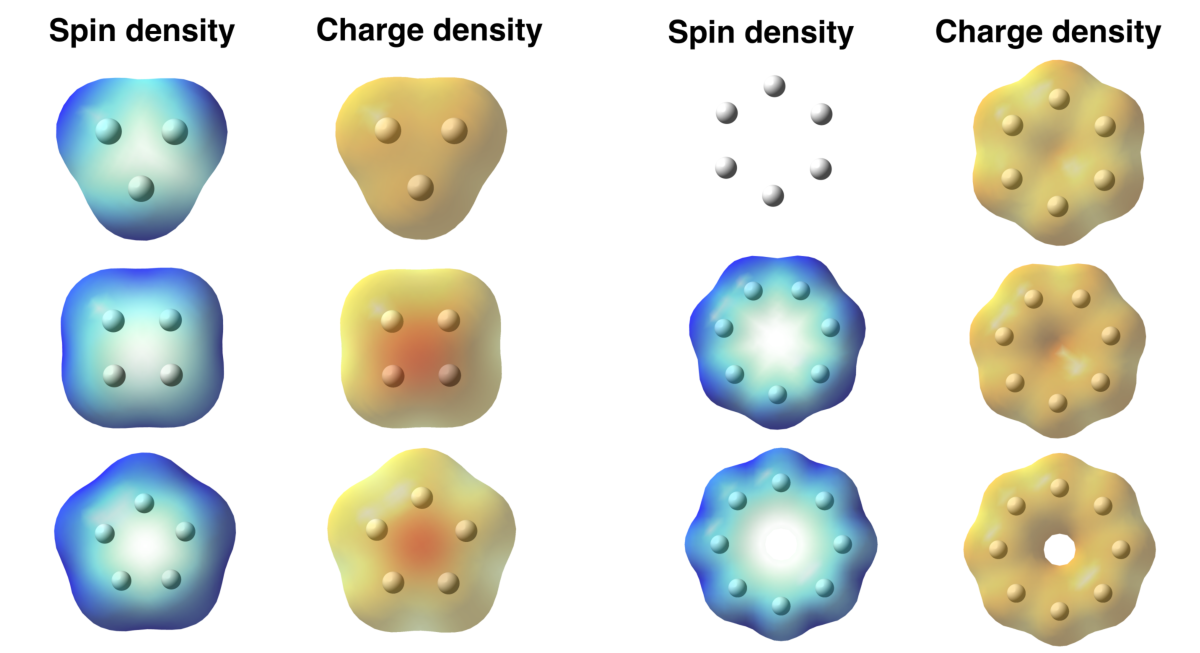
\includegraphics{rings.pdf}
}
\end{center}
\caption{X2C-B3LYP  6-311+g(D,P) spin ($\vert \vc{m}(\vc{r})\vert$, left) and scalar ($\rho^{1,0}(\vc{r})$, right) densities for a series of Hydrogen rings.
Blue and Red represent regions of greater density magnitude respectively.}
\label{fig:rings}       
\end{figure}

\subsubsection{Computational Performance}

\begin{figure}
\begin{center}
\resizebox{6.5in}{!}{%
  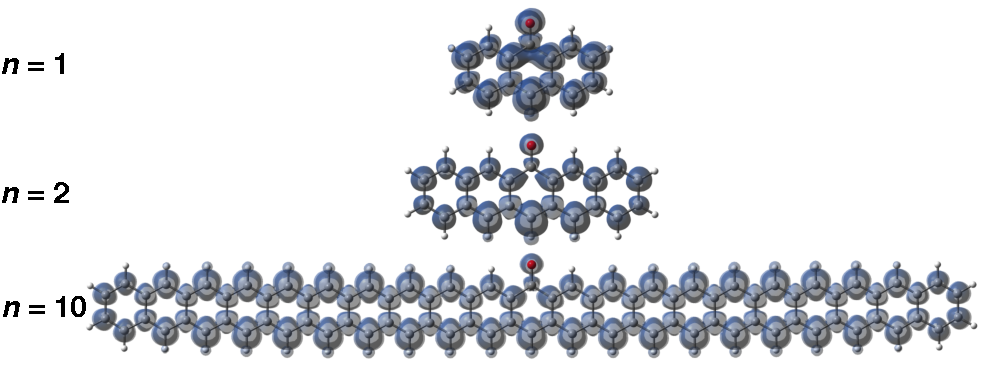
\includegraphics{radicals.pdf}
}
\end{center}
\caption{X2C-B3LYP 6-311+G(2D,P) spin densities ($\vert\vc{m}(\vc{r})\vert$) for phenoxy radicals with an increasing number of fused benzene rings 
($n$=1-10, where $n$ represents the number of fused benzene rings on each side).}
\label{fig:radicals}       
\end{figure}

In this section, we examine the computational performance of the proposed
X2C-KS method.  All the following tests presented were performed using
X2C-B3LYP/6-311+G(2D,P).  All times refer to the combined wall time for the
numerical evaluation of $ E^{GGA}$ and the matrix elements
$V^{GGA,K}_{\mu\nu}$ (\cref{eq:EXCGGA_num} and \cref{eq:VXCGGA_num}) as an
average over 5 SCF steps in the X2C-KS optimization.  

To demostrate the efficacy of our method relative to standard UKS methods,
we examine the relative scaling of UKS and X2C-KS with respect to system
size. For this numerical experiment we have choses a set of phenoxy radicals
shown in \cref{fig:radicals}. These systems were chosen as they exhibit highly
delocalized spin--density across their entire spatial extent. This allows for
a true comparison between UKS and X2C-KS as UKS will only support a particular
($z$) orientation of the magnetization vector while X2C-KS will not have this
restriction. Wall timings for single node (28 CPU core) performance on these systems are presented in \cref{fig:timings}.
As can be seen, the scaling of UKS and X2C-KS is identical with X2C-KS
having a slightly larger prefactor. In terms of raw wall timings, this increase in prefactor
does not ammount to a significant computational overhead over UKS. This is to be expected as there are (linearly)
more spin components of $\spvc V^{xc}$ is X2C-KS over UKS (per \cref{eq:DenFockConstraint}),
thus the only difference should amount to a prefactor.




To demostrate the scalability of the proposed method, we examine the parallel
performance of our implementation using the largest phenoxy radical from the
previous numerical experiment. Wall time as a function of the number of 
parallel processes utilized (1, 2, 4, 8, 12 nodes, for a total of 28, 56, 112, 224, 336 CPU cores)
for this system is are presented in \cref{fig:nodes}. The implementation of X2C-KS
is shown to exhibit linear scaling over parallel processors (a slope of -1.01).
As previously discussed in \cref{sec:NCDFT_IMPL}, this behaviour is expected
for a proper implementaion of any KS method as the operations which are to be performed
are completely independent. In out implementation, distributed memory parallelism
was achieved by placing each atomic integrand (per the Becke scheme) on
an individual MPI process while performing each atomic indegrand using shared
memory parallelism (OpenMP) of each node.

\begin{figure}
\begin{center}
\resizebox{3.25in}{!}{%
  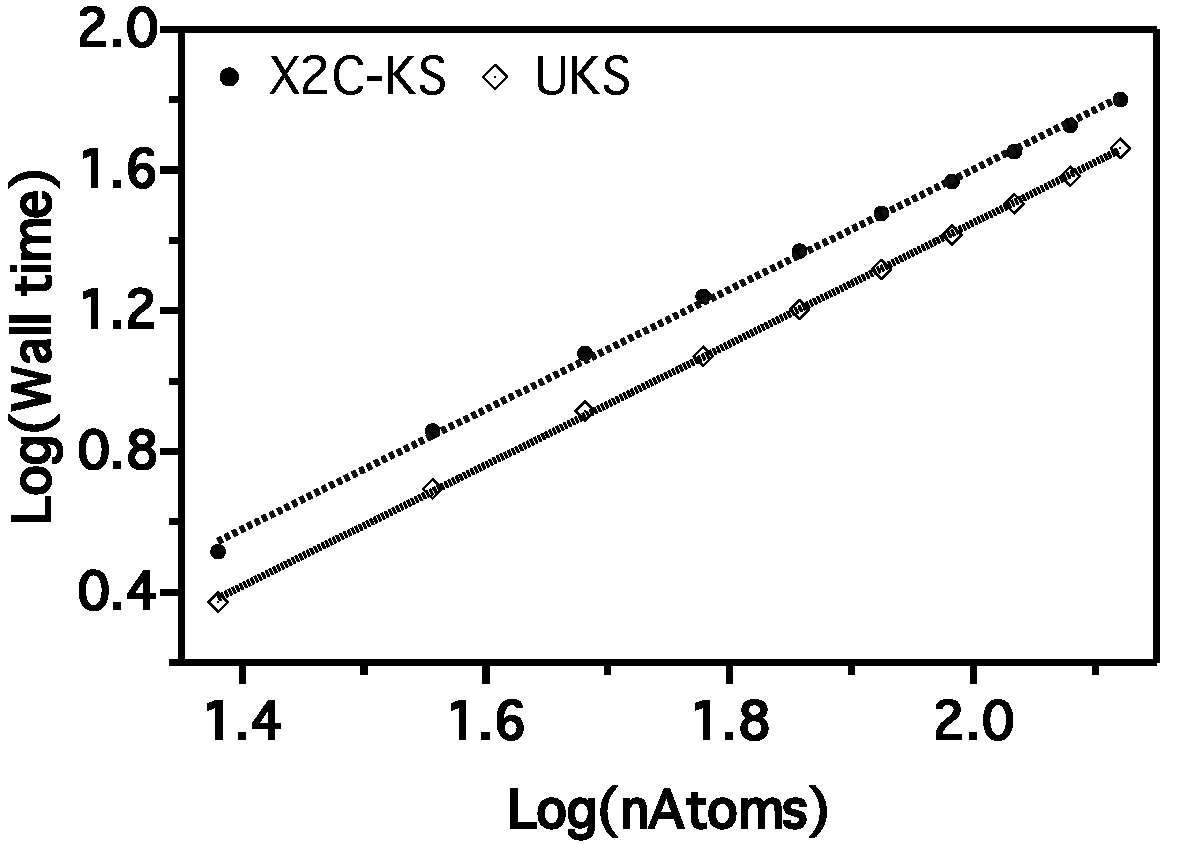
\includegraphics{timings_natoms.pdf}
}
\end{center}
\caption{
Relative scaling with respect to system size on a set of phenoxy radicals for
the UKS and proposed X2C-KS methods. Times are presented logarithmically to
demonstrate identical scaling with differing prefactors for the two methods.
Times presented are the average wall times for the numerical integration of
$E^{GGA}$ and $V_{\mu\nu}^{GGA,K}$ over 5 SCF steps.  
}
\label{fig:timing}     
\end{figure}

\begin{figure}
\begin{center}
\resizebox{3.25in}{!}{%
  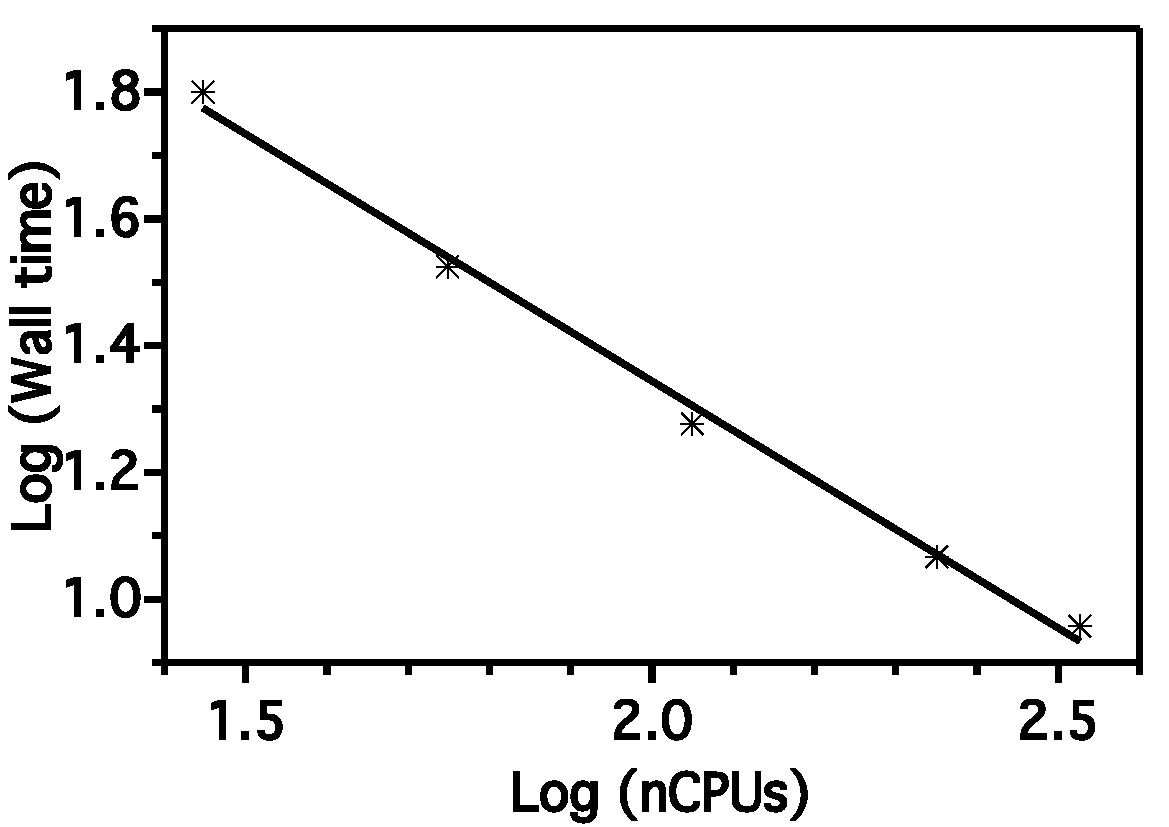
\includegraphics{cpus.pdf}
}
\end{center}
\caption{
Wall times for the distributed memory parallel performance of the proposed implementation of 
X2C-KS on a large phenoxy radical. Times are presented logarithmically to demonstrate the linear 
(-1.01) scaling of the proposed method.
Times presented are the average wall times for the numerical integration of
$E^{GGA}$ and $V_{\mu\nu}^{GGA,K}$ over 5 SCF steps.  
}
\label{fig:nodes}       
\end{figure}

\subsection{Conclusions}

In this work, we developed an efficient and scalable protocol for the
integration and assembly of the xc potential in non--collinear
KS-DFT. Initial numerical experiments demonstrate numerical stability
and robustness for the proposed method on a set of challengeing
molecular systems which exhibit non--collinearity due to geometrical
frustration. We have demonstrated excellent performance of
the proposed method both from the perspective of scaling with system
size and linear parallel scaling on distributed memory architechtures.
Further, we have shown that with the proposed algorithm, the computational 
cost relative to UKS is not significant. We hope that the proposed algorithm
will inspire development in relativistic DFT to move past proof of concept
and torwards leveraging the lastest advances in high--performance computing.




%In this work, we presented an integration and assembly strategy, 
%using a two-component spinor density, for efficient evaluation
%of the exchange correlation term using localized basis
%functions. 
%The presented formulation is suitable to exploit parallelism 
%along with optimal cache utilization and micro-architecture specific floating point operations.
%This leads to the evaluation of exchange correlation
%contributions with matrices of optimal sizes. 
%We also show that the proper choice of auxiliary variables 
%correctly give rise to nonzero local torque of the xc magnetic field on the magnetization
%while maintaining net zero global torque, as is expected from
%the exact functional. 
%Several tests were used to validate 
%the reliability and the performance of the proposed strategy.
%This approach can help to extend 
%the applicability of relativistic two-component DFT 
%to systems of large size ($>$ 100 atoms). 







\section{The Relativistic Particle--Particle Random Phase Approximation}

At times, the KS-DFT description is not sufficient for the proper description
of the electronic wave function. This case is encountered in general when
the wave function cannot be descibed properly as a single Slater determinant.
As such, in this section is oulined a two--component many--body expansion 
method (ala \cref{eq:ExcitationOp}) which includes relatativistic effects
and tackles the electron correlation problem though representing the wave function
as a linear combination of several Slater determinants. The following sections
have been adapted and reproduced with permission from David B. Williams--Young,
Franco Egidi, and Xiaosong Li. Relativistic Two--Component Particle--Particle
Tamm--Dancoff Approximation. \emph{J. Chem. Theory Comput.} \textbf{2016}, 12(11),
pp 5379-5384. Copyright 2016 American Chemical Society.




\subsection{Motivation}

The ability to accurately predict and characterize the electronically excited
states of molecular systems is paramount to a complete understanding of many
chemical phenomena. As such, excited states are the central focus of many
fields of physical chemistry, most prominent being that of spectroscopy. Due to
this centralized importance and the need to efficiently and accurately predict
excited states properties, much  effort has been devoted over the years towards
the modeling of excitation energies and oscillator strengths.


Recently, the particle-particle random phase approximation (pp-RPA) and 
Tamm-Dancoff approximation (pp-TDA), which have been standard trade tools of 
the nuclear physics community in the treatment of the many--body correlation energy for low matter density 
systems for some time \cite{SchuckBook_04}, 
have been extended to the treatment the correlation energy and excitation energies of quantum 
molecular systems within a finite basis set \cite{Yang13_224105,Yang13_18A522,
Yang13_174110,Yang13_104112,Yang13_030501,Yang09_066403,Bulik13_104113}.  Although the
introduction into the quantum chemistry community in relatively recent, a wealth 
of effort has been afforded to the rigorous investigation of these methods in a 
variety of different contexts, including the evaluation of excitation 
energies \cite{Yang13_224105,Yang13_18A522,Yang13_174110}, excited state properties 
and geometry optimizations \cite{Yang15_1025}, and the treatment of non-adiabatic 
phenomena such as non-adiabatic dynamics \cite{Liu14_244105} and the description 
of conical intersections \cite{Yang16_2407}.  So far in their development, however, 
these methods have only seen application in molecular systems using strictly 
collinear (RSCF and USCF) references, disallowing extension to systems with 
non--collinear (GSCF) reference, such as those that arise in spin-frustrated systems 
(see \cref{sec:NCDFT_VALID}) or whenever spin-orbit effects are included in the 
treatment of the electronic structure.


Recent years have also seen new developments in the realm of relativistic quantum 
chemistry.  Relativistic effects, while often neglected in most standard treatment
of electronic structure, can have profound consequences in chemical 
systems \cite{Pyykko12_45}.  Scalar relativistic effects cause the contraction of 
the core electron shells of heavy atoms, but perhaps of even more consequence is 
the introduction of spin couplings in the Hamiltonian.  Spin-spin and spin-orbit 
interactions can affect the electronic spin dynamics even in light atoms, and a 
direct consequence of these couplings on excited states is the loss of degeneracies
of spin-eigenstates, giving rise to fine structure splittings (FSS) in atoms and 
molecules with symmetry-induced degeneracies. It is therefore desirable to develop accurate and 
cost-effective relativistic electronic structure methods able to model such effects. 


Thus, in this work, we extend the pp-TDA formalism for use with 
relatvistic GSCF reference determinants, specifically the X2C-HF reference of \cref{sec:X2C,sec:MF2C}. 
However, the presented formalism may be employed in any case where the GSCF method must be
employed, such as the spin-frustrated systems explored in \cref{sec:NCDFT_VALID},
even in the absence of relativistic effects. 




\subsection{The Particle-Particle Tamm-Dancoff Approximation}
\label{subsec:ppTDA}
The pp-TDA is a non-particle-number conserving many--body expansion method, i.e. the
approximation of the excitation operator of \cref{eq:ExcitationOp} it employs does not commute with the number
operator.  To model a system with $N$ electrons, the pp-TDA starts from a
reference determinant for a system with $N-2$  electrons, and adds two
electrons back using an appropriate excitation operator.  The ground and
excited states of the $N$-particle system are thus obtained as ``excited
states'' of the $N-2$ electron reference, and the desired excitation energies
can be written as simple energy differences.  A general formalism for the
treatment of the pp-TDA within a finite basis of spin--collinear MOs has
described rigorously elsewhere
\cite{Yang13_224105,Yang13_18A522,Yang13_104112}.  Here, we review this
formalism for completeness and present the working expressions for the
relativistic X2C pp-TDA (X2C-pp-TDA) within the basis of MO spinors as well as
describe some caveats in the practical application of this method within the
context of a spinor reference.

From an (exact) $M$-particle ground state, $\ket{\Psi_0^M}$, the excitation operator
of \cref{eq:ExcitationOp} which constructs all ground and excited 
$N$-particle states ($\ket{\Psi_0^N}$ and $\ket{\Psi_n^N}$ respectively) may be written
convieniently as a projector $\op{R}^{N,M\dagger}_n = \ket{\Psi_n^N}\bra{\Psi_0^M}$, such that
\begin{equation}
  \ket{\Psi_n^N} = \op{R}^{N,M\dagger}_n \ket{\Psi_0^M}.
\end{equation}
Given such an ansatz, it is possible to construct an equation-of-motion (EOM) \cite{SchuckBook_04} 
for $\op{R}_n^{N,M\dagger}$, affording some corresponding
probing de-excitation operator $\delta \op{R}$ , to obtain the eigenenergies of $\ket{\Psi_n^N}$,
\begin{equation}
\label{eq:EOM}
  \left[ \delta \op{R},\left[ \op{H}, \op{R}_n^{N,M\dagger} \right]\right] = 
    (E^N_n - E^M_0)\left[\delta \op{R}, \op{R}^{N,M\dagger}_n \right].
\end{equation}

\Cref{eq:EOM} is formally exact and completely independent of the chosen
reference, provided one has access to the exact $N$- and $M$-particle states,
or eqivalently a closed form expression for the projector (such as \cref{eq:ExOpExp}).
In practice, one may take the expectation value of \cref{eq:EOM} using some
approximate $M$-particle ground state, which in the present work will be
a Slater determinant, $\ket{\Phi_0^M}$, to obtain
\emph{approximate} energy differences between $N$- and $M$-particle states
given some explicit (truncated) form of $\op{R}^{N,M\dagger}_n$.  As has been previously
discussed, if the $N$ and $M$ systems differ by exactly two particles ($M=N-
2$), the X2C-pp-TDA equation may be obtained by postulating that the excitation
operator take the form of all (unique) 2-particle additions to obtain
$N$-particle states from an $(N-2)$-particle reference,
\begin{equation}
  \op{R}_n^{N,(N-2)\dagger} = \sum_{a < b} X^n_{ab} \tau^{ab} , \label{eq:ppTDAExcitation}
\end{equation}
while the de-excitation operator takes the form
\begin{equation}
  \delta\op{R} = \tau_{ab}\quad.
\end{equation}
Here, $\tau$ is defined in \cref{eq:TauDef} and $X^n_{ab}$ is an expansion
coefficient that describes the contribution to the $n$-th $N$-particle state of
the addition of 2 particles into single-particle virtual states, $a$ and $b$,
of the $(N-2)$-particle ground state reference. By taking the expectation value
of \cref{eq:EOM} in a single X2C-HF Slater determinant (e.g. by using Wick's theorem) given
\cref{eq:ppTDAExcitation}, one obtains the Hermitian eigenvalue problem of the
X2C-pp-TDA
\begin{align}
\sum_{c < d} A_{ab,cd} X^n_{cd} &= \Omega_n X^n_{ab} \quad (a < b), \label{eq:ppTDA}\\
\Omega_n &= (E_n^N - E_0^{N-2}) \\
  A_{ab,cd} &= \delta_{ac}\delta_{bd} (\epsilon^\mathrm{X2C-HF}_a + \epsilon^\mathrm{X2C-HF}_b) + \innerop{ab}{r_{12}^{-1}}{cd} - \innerop{ab}{r_{12}^{-1}}{dc}  \quad \label{eq:AMat},
\end{align}
where  $\{\epsilon^\mathrm{X2C-HF}_p\}$ is the set of orbital
eigenenergies obtained from solving the X2C-HF equation in \cref{eq:X2CHFRH} and
\begin{equation}
  \innerop{ab}{r^{-1}_{12}}{cd} = \sum_{\mu\nu\lambda\kappa} \sum_{\sigma\sigma'} 
C^{\sigma*}_{\mu a}
C^{\sigma'*}_{\mu b}
C^{\sigma}_{\mu c}
C^{\sigma'}_{\mu d}
\innerop{\mu\nu}{r^{-1}_{12}}{\lambda\kappa}
\end{equation}
where $\innerop{\mu\nu}{r^{-1}_{12}}{\lambda\kappa}$ is defined in \cref{eq:ERIBasis} and $\spvc C = \spvc C^\mathrm{X2C-HF}$. 
One may obtain neutral $N$-particle excitations by examining the eigen spectrum of \cref{eq:ppTDA}. By
variationally optimizing the wave function of the $(N-2)$-particle system via
X2C-HF, both the $N$-particle ground and excited state energies are obtained
via
\begin{align}
E_n^N = E_0^{N-2} + \Omega_n \quad . \label{eq:ESEnergy}
\end{align}
Thus the excitation energy between $N$-particle ground and excited states, $\omega_n^N$, described via the X2C-pp-TDA may be written as differences of the eigenenergies,
\begin{equation}
\omega_n^N = E_n^N - E_0^N = \Omega_n - \Omega_0 \quad (n > 0). \label{eq:EXEnergy}
\end{equation}

These working expressions in \cref{eq:ppTDA,eq:AMat,eq:ESEnergy,eq:EXEnergy}
are similar to those previously expressed for the spin-collinear
reference \cite{Yang13_224105,Yang13_18A522,Yang13_104112}. The key difference
is that all of the above equations are expressed in a non--collinear GSCF spinor 
basis rather than a collinear (RSCF / USCF) orbital basis, and that the
orbitals have been optimized in the presence of relativistic spin-orbit
effects via the X2C method.
Unlike the collinear case, where significat simplification of \cref{eq:ppTDA} is
achieved through exploitation of the spin orthonality of the reference 
\cite{Yang13_224105,Yang13_174110}, the general non-collinear case presented in this
work cannot be further simplified.

\subsection{Results and Discussion}
\label{sec:ppX2CResults}

All calculations were performed with a locally modified version of the Gaussian
quantum chemistry suite of programs \cite{GDVI06}, and employed the
taug-cc-pVTZ-DK Gaussian basis set \cite{Dixon01_48} with the diffuse \emph{f}-functions
removed.  Relativistic effects were accounted for by means of the variational
X2C method outlined in \cref{sec:X2C,sec:MF2C}.
In order
to partially account for two-electron spin-orbit interaction in the
Hamiltonian, we employed a scheme based on the scaling of the nuclear charge
according to the angular momenta of the basis functions (\cref{eq:BScaling}). The atomic nuclei,
rather than being treated as point charges, were described using $s$-type
Gaussian charge distribution (\cref{eq:GauNuc}). The stability of the
two-component ground state wave function was also tested before X2C-pp-TDA
calculations were performed \cite{Li15_154109}.

\subsubsection{Single Excitations}
\label{subsec:SingleEx}
In order to highlight the capability of the pp-TDA method to describe excited
states within a relativistic framework, in this section we examine the FSS
of some atomic systems.  The presence of spin-orbit couplings 
lifts some of the energetic degeneracies that would be expected in the ground or
excited electronic states in non--relativistic theory.  
We therefore calculate the excitation energies of selected
atomic systems and compare the obtained fine structure splittings with
experimental reference values \cite{NIST_ASD} to asses the accuracy of the
method.  In this section we restrict ourselves to states describable by single
excitations (with respect to the $N$-electron system) which allows us to also
compare our results with the results obtained using the two-component
particle-hole Random-Phase Approximation (X2C-ph-RPA), also known as
Time-Dependent Hartree-Fock method (X2C-TDHF), as well as with results obtained
using the X2C-ph-TDA method \cite{Li16_3711}. Results for these FSS estimations 
are collected in \cref{tb:SingleEx}.

It can be seen that, in general, the three methods perform similarly with
respect to the reference values insofar as the order of magnitude of the error
is concerned. A general trend may be observed in that the X2C-pp-TDA
consistently overestimates the splittings as the atomic charge of the
underlying nucleus increases. This effect is magnified in the low energy
transitions while it is less apparent in the higher energy transitions. This is
due to the fact that the frontier orbitals of the ($N-2$)-reference being used
become sub-optimal in the proper description of the $N$-electron system due to
a contraction in the presence of higher nuclear charge. This leads to an
unphysically small energetic separation between the frontier orbitals of the
$N$-electron system which causes increasing errors due to an unphysical
increase in mixing. This problem is less obvious in higher energy excitation
because the higher lying orbitals are not as affected. These orbitals are
properly optimized in the X2C-ph-RPA/TDA due to orbital occupancy of the
resulting wave function. The general out-performance of the X2C-ph-TDA over the
X2C-ph-RPA may be attributed to an over estimation of electron correlation in
the ground and excited states via the RPA \cite{Dreuw05_4009}. The presence of
the de-excitation amplitudes in the X2C-ph-RPA allow for an over-mixing for the
low-lying excited states with the ground state which give rise to an
overestimate of the FSS, much the same as the case for the X2C-pp-TDA.
                                                                                                                                                 
 
                                                                                                                                                                                                                                                              
 
The main advantage of the particle-particle over the particle-hole formalism is
that, in the former, both the ground and electronically excited $N$-particle
states are described on equal footing with respect to correlation, being a
linear combination of several Slater determinants.  Conversely, in the ph-TDA
or ph-RPA method, the ground state is described as a single determinant, while
excited states are described as linear combinations of single excitations (and
possibly de-excitations).  That being said, the excitation space spanned by the
X2C-pp-TDA solutions does not include all chemically relevant excitations, many
of which can be found using the more traditional ph-RPA or ph-TDA methods.
This is due to the fact that the X2C-pp-TDA is, in its traditional form,
incapable of accessing excitations that involve contributions from below the
Fermi level.  Some work has been done in attempts to resolve this
problem \cite{Yang13_224105}, but these alterations to the pp-TDA method have
not been explored in this work.

\begin{table}[htbp]
  \caption{Calculated and reference \cite{NIST_ASD} excited-state fine structure splittings (in meV) for 
  single excitations of some atomic systems. The presence of a superscript ``$\circ$" in the term symbol 
  denotes an odd state with respect to space inversion.}
 \label{tb:SingleEx}
 \centering
 \begin{tabular}{llrrr}
  \hline
  Method     & Level                                              &  Mg   & Al$^+$ & Si$^{2+}$ \\ \hline
  X2C-ph-RPA & \multirow{3}{*}{$^3$P$^\circ_{1}-^3$P$^\circ_{0}$} &  4.89 & 10.49  & 19.85 \\
  X2C-ph-TDA &                                                    &  2.41 &  7.94  & 16.62 \\
  X2C-pp-TDA &                                                    &  2.77 &  9.13  & 18.97 \\
  Ref        &                                                    &  2.49 &  7.55  & 15.94 \\
  \hline
  X2C-ph-RPA & \multirow{3}{*}{$^3$P$^\circ_{2}-^3$P$^\circ_{1}$} &  9.75 & 21.02  & 39.96 \\
  X2C-ph-TDA &                                                    &  4.82 & 15.96  & 33.50 \\
  X2C-pp-TDA &                                                    &  5.55 & 18.40  & 38.40 \\
  Ref        &                                                    &  5.05 & 15.36  & 32.45 \\
  \hline
  X2C-ph-RPA & \multirow{3}{*}{$^3$P$^\circ_{1}-^3$P$^\circ_{0}$} &  0.33 &  1.82  &  4.43 \\
  X2C-ph-TDA &                                                    &  0.33 &  1.82  &  4.31 \\
  X2C-pp-TDA &                                                    &  0.42 &  2.17  &  5.08 \\
  Ref        &                                                    &  0.41 &  1.73  &  4.10 \\
  \hline
  X2C-ph-RPA & \multirow{3}{*}{$^3$P$^\circ_{2}-^3$P$^\circ_{1}$} &  0.67 &  3.67  &  9.09 \\
  X2C-ph-TDA &                                                    &  0.67 &  3.68  &  8.86 \\
  X2C-pp-TDA &                                                    &  0.84 &  4.50  & 11.04 \\
  Ref        &                                                    &  0.84 &  3.65  &  9.07 \\ 
  \hline
  \\
  \\
             &  &  MSE  &  MAE   & \\
  \hline
  X2C-ph-RPA &  &  2.32 &  2.28  & \\
  X2C-ph-TDA &  &  0.32 &  0.19  & \\
  X2C-pp-TDA &  &  1.55 &  1.55  & \\
  \hline
 \end{tabular}
\end{table}

\subsubsection{Triplet References and Double Excitations}
\label{subsec:DoubleEx}
In this section we wish to highlight other advantages of X2C-pp-TDA over
conventional X2C-ph-RPA.  In the previous section we presented results for
atomic systems that are characterized by being closed shell in both the $N$ and
$N-2$ systems.  This is important because if the reference state has unpaired
electrons then, as a consequence of the single reference nature of the
Hartree-Fock wave function, excited states will in general be
spin-contaminated, affecting one's ability to extract meaningful fine structure
splittings from the results, though adaptations to remedy this problem in the 
general case exist \cite{Liu10_064106,Suo11_134101,Liu11_194106,Liu12_024107,Liu13_3741}. By
using X2C-pp-TDA it is possible to treat systems with $N$ electrons
with any odd spin multiplicity, provided they become closed shell upon the
addition or removal of two electrons.  Molecules which possess triplet ground
states as well as diradical moieties may be taken as examples.  To demonstrate
this feature we compare the FSS of one set of excited states of molecular
oxygen with experimental data in \cref{tb:DoubleEx}.  The difference between
the calculated and measured value is just 2.5~meV, notwithstanding the
approximations intrinsic in our method (e.g.~the approximate treatment of
electron correlation and the two-electron spin-orbit contributions, or the
finite basis set).  Of course, the same reasoning can also be applied in
reverse: X2C-ph-RPA theory can be readily used to find excited-state FSS of
systems with a singlet ground state, however if the addition or removal of two
electrons produces an open-shell molecule, then X2C-pp-TDA will present some
spin-contamination in the computed excited-states.



One advantage that X2C-pp-TDA always has over X2C-ph-RPA theory, however, is
its ability to describe double excitations.  \Cref{tb:DoubleEx} compares
calculated and reference excited-state FSS of doubly-excited states of some
atomic moieties.  The performance of the method is similar as in the case of
single excitations presented in the previous section.  Such states cannot be
found among the excited states computed via X2C-ph-RPA.

\begin{table}[htbp]
 \caption{Excited-state fine structure splittings (in meV) for triplet
  and doubly excited electronic states calculated by the X2C-pp-TDA method.}
 \label{tb:DoubleEx}
 \centering
 \begin{tabular}{llrr}
  \hline
  System & Level & X2C-pp-TDA & Ref \cite{NIST_ASD,Krupenie72_423} \\ \hline
  O$_2$ & $^3\Delta_3-{^3\Delta_2}$ & 20.58 & 18.09 \\ \hline
  \multirow{2}{*}{Al$^+$} & $^3$P$_1-^3$P$_0$ & 9.20 & 7.75 \\ 
  & $^3$P$_2-^3$P$_1$ & 17.93 & 15.03 \\  \hline
  \multirow{2}{*}{Si$^{2+}$} & $^3$P$_1-^3$P$_0$ & 19.46 & 16.55 \\ 
  & $^3$P$_2-^3$P$_1$ & 37.88 & 32.06 \\    \hline
 \end{tabular}
\end{table}

%-------------------------------------------------------------------------------
% CONCLUSION
%-------------------------------------------------------------------------------
\subsection{Conclusion}

In this work, a scheme for the extension of the pp-TDA method to relativistic
two-component wave functions has been presented.  This scheme involves the
approximate decoupling of the large and small components of the relativistic
wave function by means of the X2C method, followed by an Hartree-Fock SCF
calculation on the system obtained by removing two electrons, in order to
obtain a set of complex spinor molecular orbitals.  The two-component reference
system is then used in the X2C-pp-TDA calculation that yields the ground and
excited states for the $N$-electron system.  The extension of the pp-TDA to a
two-component reference comes at the cost of the employing complex spinor
orbitals, and not being able to separate the problem into smaller sub-problems
as is done in the case of RHF or UHF references via spin integration.  The
increased computational cost highlights the ever pressing need for direct and
parallel implementations of post-SCF electronic structure methods, which is
exaggerated in the case of relativistic electronic structure calculations.

It has been shown that the X2C-pp-TDA method exhibits excellent results in the
prediction of the fine-structure splittings of the atomic and molecular species
considered here.  The results are comparable and at times better than those
obtained using X2C-ph-RPA \cite{Li16_3711}. In addition, the X2C-pp-TDA is able
to capture electronic excitations traditionally inaccessible by the
X2C-ph-RPA/TDA thanks to the 2-particle reference shift, such as double
excitations and those that would be described as spin-contaminated in
particle-number conserving methods.  While these results are promising, the
general applicability of the X2C-pp-TDA method, as with the spin-collinear
variant, is limited as it is traditionally unable to capture excitations that
involve contributions of orbitals from below the Fermi level.  That being said,
there are many systems, such as triplet and diradical systems, that the
X2C-pp-TDA provides a suitable method for the accurate description of the
electronic manifold.

